\section{Method}
\subsection{System overview}

TODO: figure of system diagram (FSM + RAM):
\begin{figure}
    \centering
    \includegraphics[width=0.5\linewidth]{}
    \caption{System diagram}
    \label{fig:03:system_diagram}
\end{figure}

Our system consists of a Finite State Machine and a Random Access Memory, as can be seen in \ref{fig:system_diagram}. The FSM serves as a control unit to make sure all operations on the RAM are performed in a stable manner. The FSM is connected to a clock signal, but the RAM is not directly, only indirectly through being controlled by the FSM.

\subsection{RAM}
The RAM subsystem concists of bitcells forming bytecells that stack on top of each other to form the full memory. It takes in as inputs:
\begin{itemize}
    \item 
    \item adr - an address signal
\end{itemize}

\subsubsection{The bitcell}

\subsubsection{The bytecell}

\subsubsection{Final layout}


\subsection{FSM}
The finite state machine is meant to 

\subsubsection{Circuit design}




\begin{figure}
    \centering
    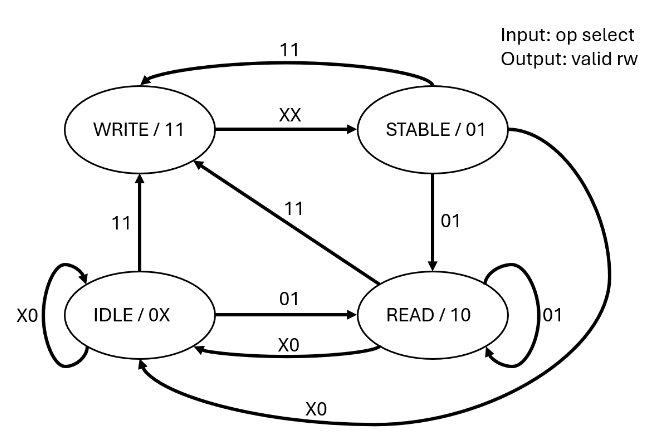
\includegraphics[width=0.7\linewidth]{LaTeX_2/Figures/state_diagram.png}
    \caption{Desired state diagram \cite{oppgavebeskrivelse}}
    \label{fig:03:state_diagram}
\end{figure}

\begin{table}[]
    \label{tab:03:state_code}
    \caption{State code and their meaning.}
    \centering
    \begin{tabular}{|l|c|}
        \hline
        State   &   Code    \\  \hline
        IDLE    &   0 X     \\  
        STABLE  &   0 1     \\
        READ    &   1 0     \\
        WRITE   &   1 1     \\  \hline
    \end{tabular}
\end{table}


\begin{table}[]
    \label{tab:FSM_truth_table}
    \caption{Truth table for Finite State Machine.}
    \centering
    \begin{tabular}{|cc|cc|cc|cc|}
        \hline
        \multicolumn{2}{|l|}{State} & \multicolumn{2}{l|}{Input} & \multicolumn{2}{l|}{State nxt} & \multicolumn{2}{l|}{Output}        \\ \hline
                     &              & Op          & Sel          &                &               & Valid & R/W \\
        A            & B            & C           & D            & E              & F             & G     & H                          \\ \hline
        0            & 0            & 0           & 0            & 0              & X             & 0     & X                          \\
        0            & 0            & 0           & 1            & 1              & 0             & 0     & X                          \\
        0            & 0            & 1           & 0            & 0              & X             & 0     & X                          \\
        0            & 0            & 1           & 1            & 1              & 1             & 0     & X                          \\
        0            & 1            & 0           & 0            & 0              & X             & 1     & 0                          \\
        0            & 1            & 0           & 1            & 1              & 0             & 1     & 0                          \\
        0            & 1            & 1           & 0            & 0              & X             & 1     & 0                          \\
        0            & 1            & 1           & 1            & 1              & 1             & 1     & 0                          \\
        1            & 0            & 0           & 0            & 0              & X             & 0     & 1                          \\
        1            & 0            & 0           & 1            & 1              & 0             & 0     & 1                          \\
        1            & 0            & 1           & 0            & 0              & X             & 0     & 1                          \\
        1            & 0            & 1           & 1            & 1              & 1             & 0     & 1                          \\
        1            & 1            & 0           & 0            & 0              & 1             & 1     & 1                          \\
        1            & 1            & 0           & 1            & 0              & 1             & 1     & 1                          \\
        1            & 1            & 1           & 0            & 0              & 1             & 1     & 1                          \\
        1            & 1            & 1           & 1            & 0              & 1             & 1     & 1                          \\ \hline
    \end{tabular}
\end{table}




\begin{align*}
    E   &=  D \cdot \overline{A \cdot B}   \\
    F   &=  A \cdot B + C \cdot D     \\
    G   &=  B                             \\
    H   &=  A
    \label{eq:03:boolean_equation}
\end{align*}